\chapter{Introduction}
Technological studies in the fields of \gls{adas} and \gls{ad} have been substantially growing in the past decades in the auto-mobile industry and in the academic environment. 

An electric car platform equipped with sensors can be programmed to have the sensation of perception. It is important for \gls{ad} vehicles to actuate accordingly to their environment. This thesis is focused on the research of a method to segment data into labels using a camera and \gls{lidar} sensors in ATLASCAR 2, so that the vehicle can later create a model of the objects it will detect, track and label.

The objects detected by ATLASCAR 2 are to be used in deep-learning algorithms. The acquired data must be large enough so that the models for each object can be well defined.

This dissertation will focus on an improvement on the calibration of the camera installed in ALTASCAR 2. In addition to the calibration, a tool for image labeling and tracking of objects will be developed. This tool will be used to gather image templates while tracking objects in the camera video. 

\section{ATLAS Project}

ATLAS is a project created by the Group of Automation and Robotics at the Department of Mechanical Engineering of the University of Aveiro, Portugal. The mission of the ATLAS project is to develop and enable the proliferation of advanced sensing and active systems designed for implementation in automobiles and affine platforms. Advanced active systems being improved, or newly developed, use data from vision, laser and other sensors. The ATLAS project has vast experience with autonomous navigation in controlled environments and is now evolving to deal with real road scenarios. To ensure that the developments are meeting the ATLAS project mission statement, a full sized prototype, the ATLASCAR 1, has been equipped with several state of the art sensors. \cite{LARlabs} Currently, ATLASCAR 2 is the new full sized prototype being used for research. The ATLASCAR 2 is also equipped with \gls{lidar} sensors and a camera.

\subsection{History}

The ATLAS Project was created in 2003 and began with robots developed to participate at \gls{ad} competitions taking place at Portuguese National Robotics Festival. From this project, three small-sized platform robots were built (figure \ref{fig:atlasproto}). These robots were very successful having won prizes in some of the robotics competitions. 


\begin{figure}[htp]
	
	\centering
	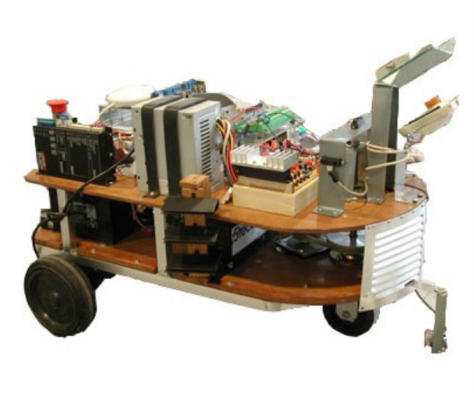
\includegraphics[width=.3\textwidth]{capintro/imgs/atlas1}\hfill
	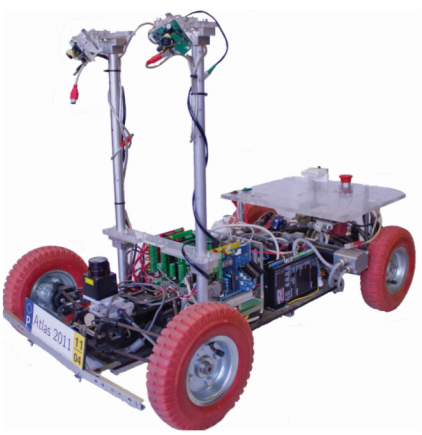
\includegraphics[width=.3\textwidth]{capintro/imgs/atlas2000}\hfill
	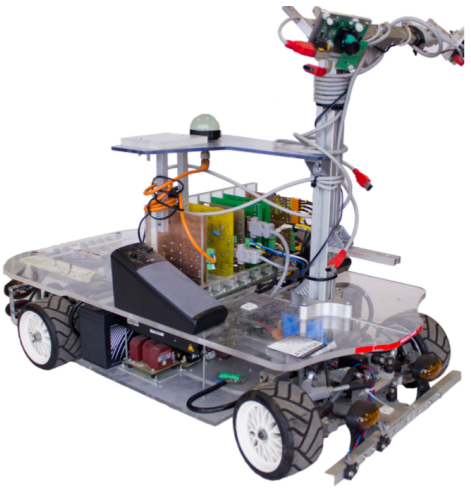
\includegraphics[width=.3\textwidth]{capintro/imgs/atlasmv}
	
	\caption{ATLAS project small-sized prototypes}
	\label{fig:atlasproto}
	
\end{figure}

As the project grew, it has evolved into full-sized prototypes: the ATLASCARs. ATLASCAR 1 (figure \ref{fig:atlascar1}) is the first full-sized platform and it is based on a Ford Escort Station Wagon. The ATLASCAR 1 is well equipped with several \gls{lidar} sensors and a camera. Data about its environment is gathered by the scanners which is then processed building perception into the car. With perception is possible for the vehicle to actuate allowing the car to move autonomously. 

\begin{figure}[htp]
	
	\centering
	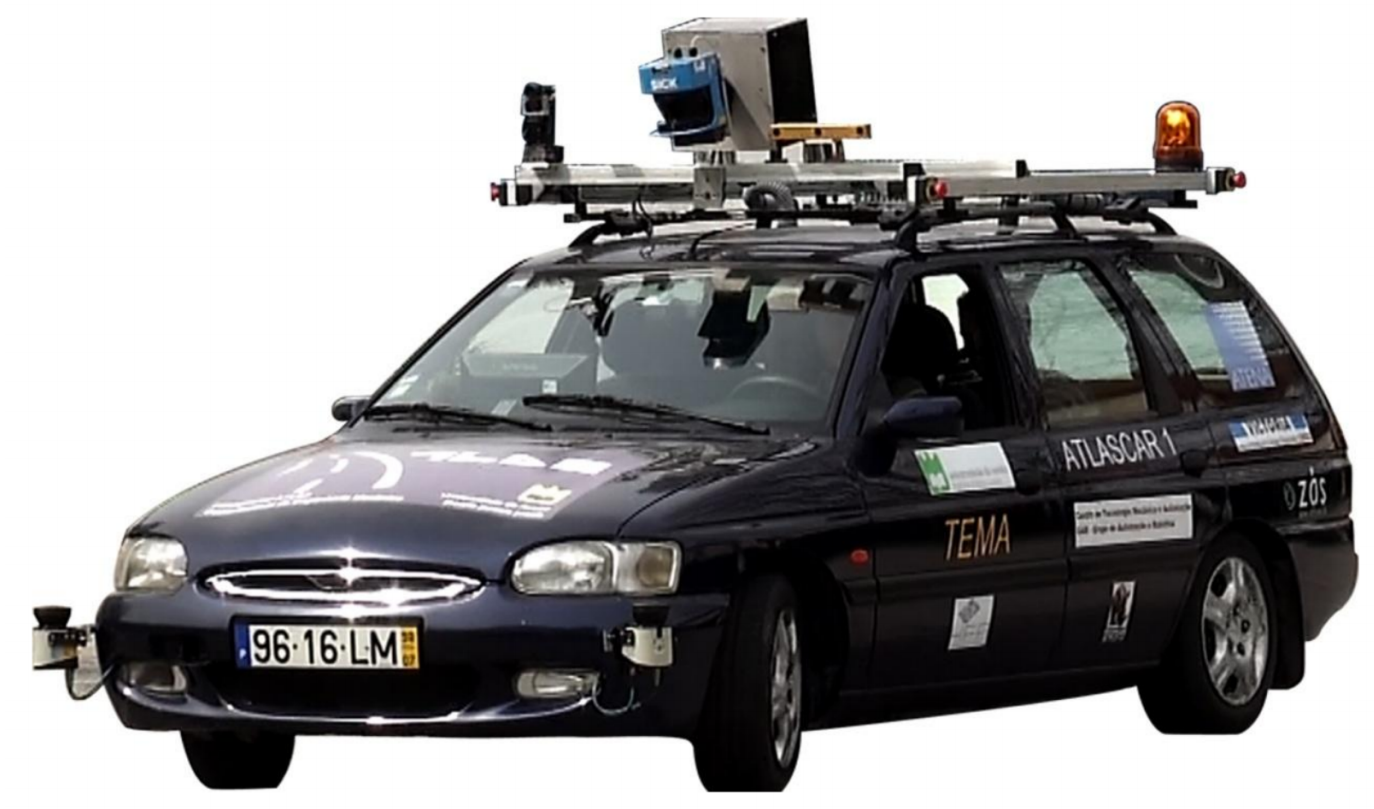
\includegraphics[width=0.9\textwidth]{capintro/imgs/atlascar1}
	
	\caption{ATLASCAR 1 based on the Ford Escort platform}
	\label{fig:atlascar1}
	
\end{figure}

The ATLASCAR 1 brought successful results. In the end, the vehicle was able to move and execute maneuvers autonomously in small and controlled places. The ATLASCAR 1 was then replaced by a more recent vehicle. The ATLASCAR 2 (figure \ref{fig:atlascar1}) is the new full-sized platform of the ATLAS project and it is based on a Mitsubishi i-MiEV. This is the vehicle used for research in this dissertation. The ATLASCAR 2 is well equipped with various \gls{lidar} sensors and a camera. It is also a full electric vehicle which will be easier to modify, test and control. 

\begin{figure}[htp]
	
	\centering
	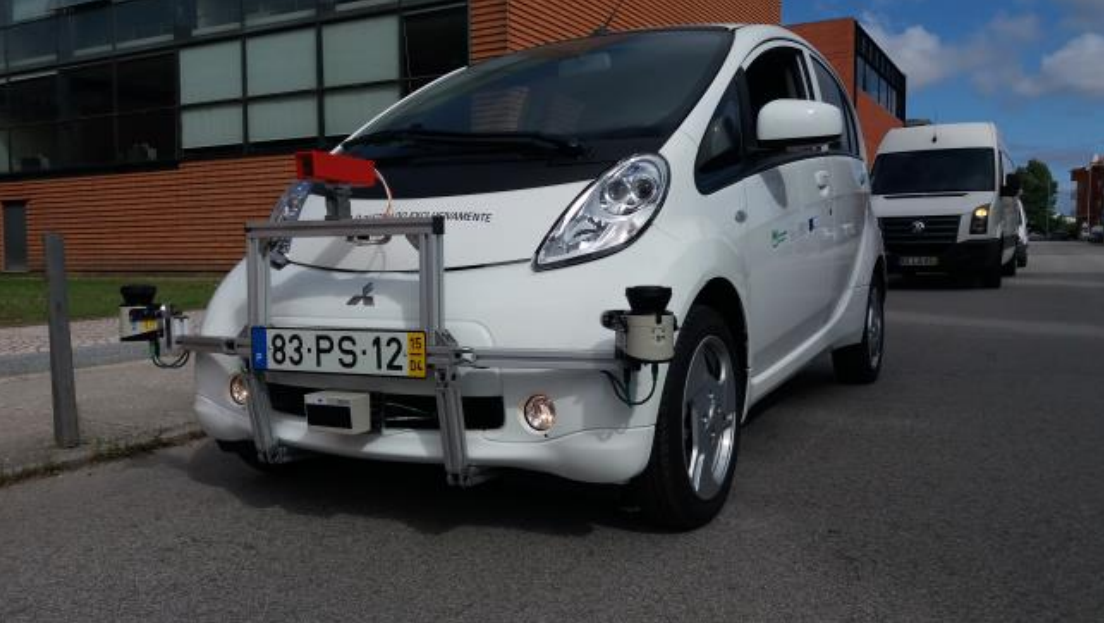
\includegraphics[width=0.9\textwidth]{capintro/imgs/atlascar2}
	
	\caption{ATLASCAR 2 based on the Mitsubishi i-MiEV platform}
	\label{fig:atlascar2}
	
\end{figure}


\subsection{Related work on ATLASCAR2}

\gls{ad} and \gls{adas} are trendy topics at \gls{lar} in the University of Aveiro. Some research on the ATLASCARs related to \gls{ad} has been made in the past. There are some relevant dissertations done at \gls{lar} that were useful for this project. 

\subsubsection{Multisensor Calibration and Data Fusion Using LIDAR and Vision} 

This is a master's thesis made by Silva \cite{VieiradaSilva2016}. The work presents an expansion to an existing extrinsic calibration package to vision-based sensors where a ball is used as calibration target. 

The calibration consists in a appearance-based algorithm to detect the ball in the image and a range-based algorithm to detect the ball in the surroundings. 

The calibration package consists in a graphical interface that allows the user to configure the various sensors to be calibrated. The estimated positions between sensors are achieved with sensor data fusion.

\subsubsection{Visual and Depth Perception Unit for	ATLASCAR2} 

This is a master's thesis made by Correia \cite{Correia2017}. It is focused on the installation of an aluminum infrastructure on ATLASCAR 2 to support ranging and vision-based sensors. The sensors setup also include the electrical project in which a power distribution circuit was developed, consisting in the wiring installation and the communication infrastructure. 

In addition, sensor calibration was done using the calibration graphical interface developed by Silva \cite{VieiradaSilva2016}. New sensors were added to the package so that the calibration could be proceeded. To demonstrate the functionalities of the platform setup, a multisensor data merging application was developed representing the free space to navigate around the car.

\subsubsection{Active Tracking of Dynamic Multivariate Agents} 

This is a PhD Thesis made by Almeida \cite{SoaresDeAlmeida2016a}. The thesis is based in \gls{mtt} in the fields of advanced safety systems. The focus lies in the prediction of the movement and actions of external agents. Two main targets are studied: vehicles and pedestrians. 

This thesis proposes techniques to improve motion prediction to achieve the development of algorithms capable of target tracking. These algorithms make use of the 3D point clouds of the environment and vision-based sensors. 


\section{Motivation}
The ATLASCAR 2 is the new platform of the ATLAS Project. The car has a mounted infrastructure for \gls{lidar} scanners and a vision-based sensors. With a fully equipped vehicle, the data from the surroundings is ready to be received and processed.

\section{Objectives}
The objectives for this dissertation are, firstly, to improve the calibration of the camera, in particular regarding the detection of the ball by the camera in the existing multi-sensor calibration package developed using the \gls{ros}. Secondly, the development of other \gls{ros} package used for semi-automatic detection and labelling of objects in the field of view.

The calibration package was already developed by Silva\cite{VieiradaSilva2016}. The methods used to detect the ball in the camera image were basically filtering  values from the \gls{hsv} color space. There are methods that can make this detection more robust that will be explained in this thesis. 

To complete the goal of object tracking and image labelling there were a set of techniques and libraries used. In vision-based sensors, the object tracking algorithm is based on template matching methods and in range-based sensors the tracking is accomplished by the \gls{mtt} library developed by Almeida \cite{SoaresDeAlmeida2016a}.

\section{Document Structure}

Escrever estrutura do documento quando este estiver completo

